
% \section{Introduction}
% OPENING - DEMOCRACY 
Democracies face two big problems. First, they are vulnerable to fleeting passions and demagogues. To combat this, they leave many decisions to experts who, ideally, use wisdom and judgment loosely guided by the public. Second, everyone cannot vote on every decision. Thus, they delegate power to representatives (who then delegate it to deputies), create temporary mini-publics,
and solicit input from those most affected or moved by a public decision.\footnote{
As imagined by \citet{Dahl1989}, mini-publics are representative, selected at random, and deliberative. Besides juries, however, deliberative and randomly-selected bodies are rare. Instead, citizens more often engage in government decisions when given opportunities to opt-in, such as hearings, petitions, and public comment periods. These mechanisms of engagement generate a different, more contentious flavor of public input than the discourse imagined by scholars who focus on deliberation.
}
Most policy is then made by bureaucrats, supposedly guided indirectly through elected representatives and directly by limited public input (mostly limited to highly contentious policy debates).
By one estimate upward of 90\% of legally binding U.S. federal policy is now written by agencies \citep{West2013}.

% Both of these problems converge in the bureaucracy, run by experts who are deputized by elected officials (or by their deputy's deputy's deputy) and with procedures that create opportunities for public input. It is far from clear how bureaucratic decisions are to balance expertise, accountability to elected officials, and responsiveness to public input in decisionmaking. 


% \subsection{Why study rulemaking?}
% \section{The Importance of Studying Rulemaking}
% Mobilization may increasingly target rulemaking because it is how most policy in the U.S. is now made. 
With the rise of the administrative state in the United States, federal agencies have become a major site of policymaking and political contestation. In the years or decades between legislative enactments, federal agencies make legally-binding rules interpreting and reinterpreting old statutes to address emerging issues and priorities. %Ninety percent of new policy that carries the force of law is now made in the bureaucracy rather than in Congress \citep{West2013WhoControl}.\footnote{I use policy, law, and regulation as nested concepts. My methods generally apply to all policy texts whether they carry the force of law or not. Many public and private organizations, including agencies, have policy statements that are not legally binding. My empirical subject is rules that do carry the force of law based on some authorizing legislation. I use rule (a more technical term) and regulation (a more colloquial term) interchangeably.}
Examples are striking: The effect of the Dodd-Frank Wall Street Reform and Consumer Protection Act was largely unknown until the specific regulations were written, and it continues to change as these rules are revised. 
Congress authorizes billions in farm subsidies and leases for public lands, but who gets them depends on agency policy. In the decades since the last major environmental legislation, agencies have written thousands of pages of new environmental regulations and thousands more changing tack under each new administration. Agency rules are revised more often than legislation \citep{Wagner2017}. And these revisions can significantly shape lives and fortunes. For example, in 2006, citing the authority of statutes last amended in the 1950s, the Justice Department's Bureau of Prisons proposed a rule restricting eligibility for parole. In 2016, the Bureau withdrew this rule and announced it would be requiring fewer contracts with private prison companies, precipitating a 50\% loss of industry stock value. Six months later, a new attorney general announced these policies would again be reversed, leading to a 130\% increase in industry stock value. %Like many rulemaking debates, industry and advocacy groups spent millions of dollars lobbying on this issue. Few rulemakings, however, receive this level of public and presidential attention. In the majority of rulemakings, few participate, and we do not really know the extent to which participants get what they lobby for.% (but see Yackee and Yackee 2006)
Rulemaking clearly matters.

Less clear, however, is how the new centrality of agency rulemaking fits into American democracy. In addition to the complex relationships agencies have with the president and Congress, agencies have complex and poorly understood relationships with the public and advocacy groups. Relationships with constituent groups may even provide agencies a degree of ``autonomy'' from their official principals \citep{Carpenter2001}. 

Expertise, delegation, and limited public input converge in bureaucratic policymaking, where bureaucrats are required to use reasoned judgment, be accountable to elected officials, and be responsive to public input. There is no normative consensus on how to rank or merge these aims.
Administrative procedures for gathering public input and their justifications cite all three.

While some suggest that requirements for agencies to solicit and respond to public comments on proposed rules allows ``civil society'' to provide public oversight, others note that participants in rulemaking often represent elites \citep{Seifter2016UCLA} and business interests \citep{Yackee2006JOP}. 

Yet agency decisions are also the target of advocacy campaigns.\footnote{For example, along with 50 thousand protesters in Washington D.C., the State Department Received 1.2 million comments on the Environmental Impact Statement for the Keystone Pipeline. Similarly, along with the thousands of protesters supporting the Standing Rock Sioux protest to the Dakota Access Pipeline, the Army Corps of Engineers received hundreds of thousands of comments. Alongside protest actions that included shutting down many websites, the Federal Communications Commission's open internet rule received 22 million comments. %On each of these issues, advocacy activity has been followed by legislative or executive action.
} 
While most rules receive little attention, the ease of online mobilizing and commenting has created exponential increases in the number of rules in which thousands, or even millions of people engage (see figure \ref{fig:comments}).\footnote{Proposed rules that have attracted the most public attention have been published by the Federal Communications Commission (FCC, omitted from this plot), the Environmental Protection Agency (EPA), the Department of Interior (DOI), the Bureau of Ocean Energy Management (BOEM), the Consumer Financial Protection Bureau (CFPB), and Fish and Wildlife Service (FWS).} Occasionally, a large number of people are paying attention.

Agencies advertise public comment periods as an opportunity for a voice in government decisions.\footnote{
% FOCUS
I focus on public comments in rulemaking, but my theory and methods also apply to other kinds of political engagement such as through social media or protests as well as to other political decisions, including state-level rulemaking. Social media engagement may be especially important if agencies implement the recommendations of \citet{ACUS2018} that ``Agencies should consider using social media before or in connection with direct final rulemaking to quickly identify whether there are significant or meaningful objections'' (p. 34). 
} 
%The notice-and-comment process purports to be an avenue of citizen voice. 
Big red letters across the top of the Regulations.gov homepage solicit visitors to ``Make a difference. Submit your comments and let your voice be heard'' (Figure \ref{fig:regs.gov}). A blue "Comment Now!" button accompanies a short description of each draft policy and pending agency action. 
Public commenting on proposed agency rules is described as ``an important part of democracy'' (WSJ 2017), the ``purest example of participatory democracy in actual American governance'' \citep{Herz2016}. \citet{Rossi1997} finds that ``courts, Congress, and scholars have elevated participation [in rulemaking] to a sacrosanct status...greater participation is generally viewed as contributing to the democracy.'' % Is it?

\begin{figure}'
    \centering
    \caption{Regulations.gov Solicits Public Comments on Draft Agency Rules}
    \label{fig:regs.gov}
    
\includegraphics[width= 5in]{regulations-header.png}
\end{figure}



\begin{figure}
\caption{Number of Public Comments per Rule 2006-2017.}
\centering
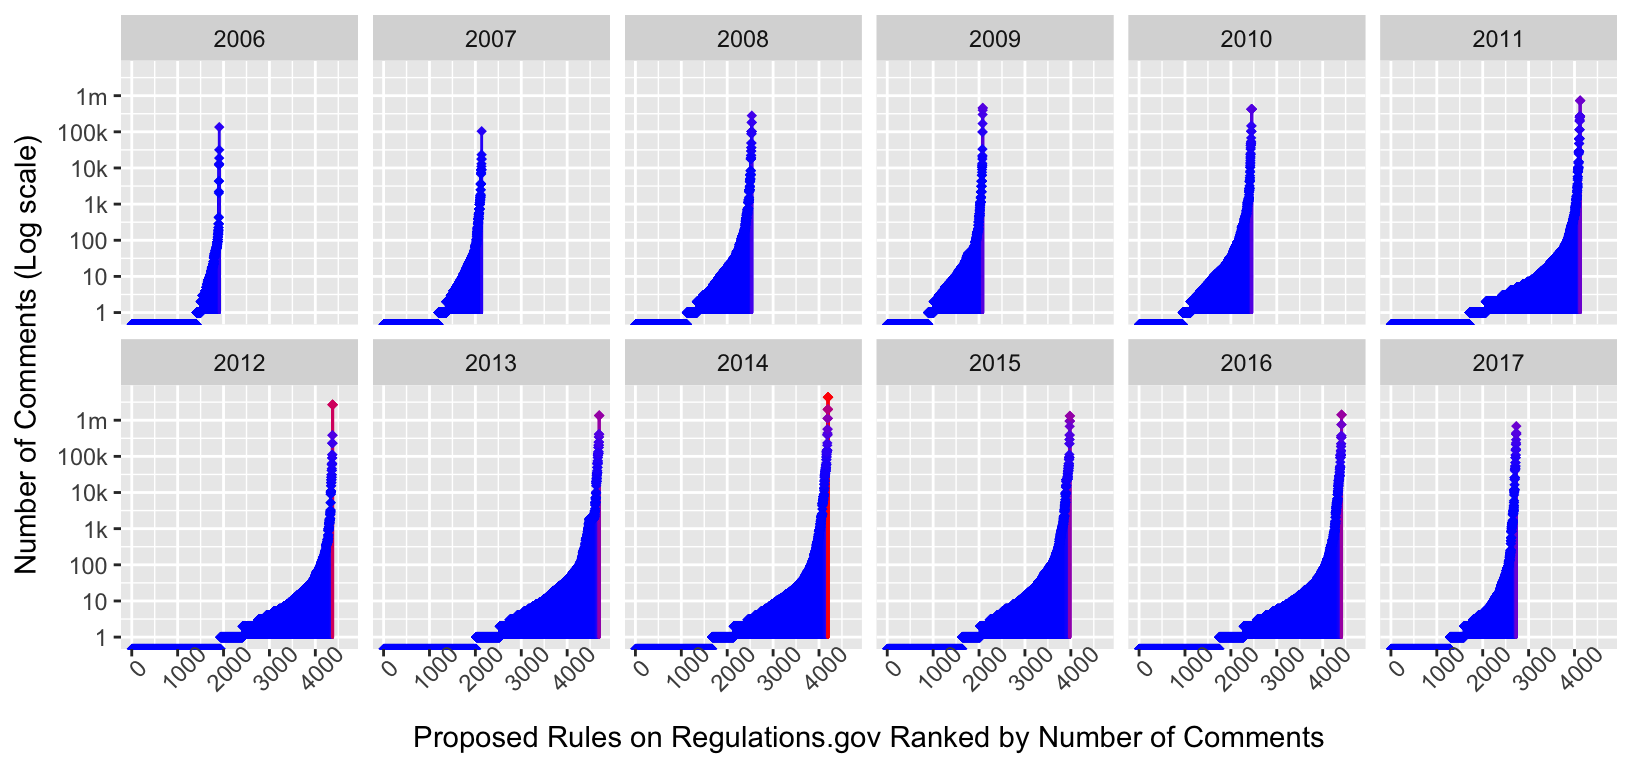
\includegraphics[width= 6.5in]{Figs/comments-per-year-1.png}
% 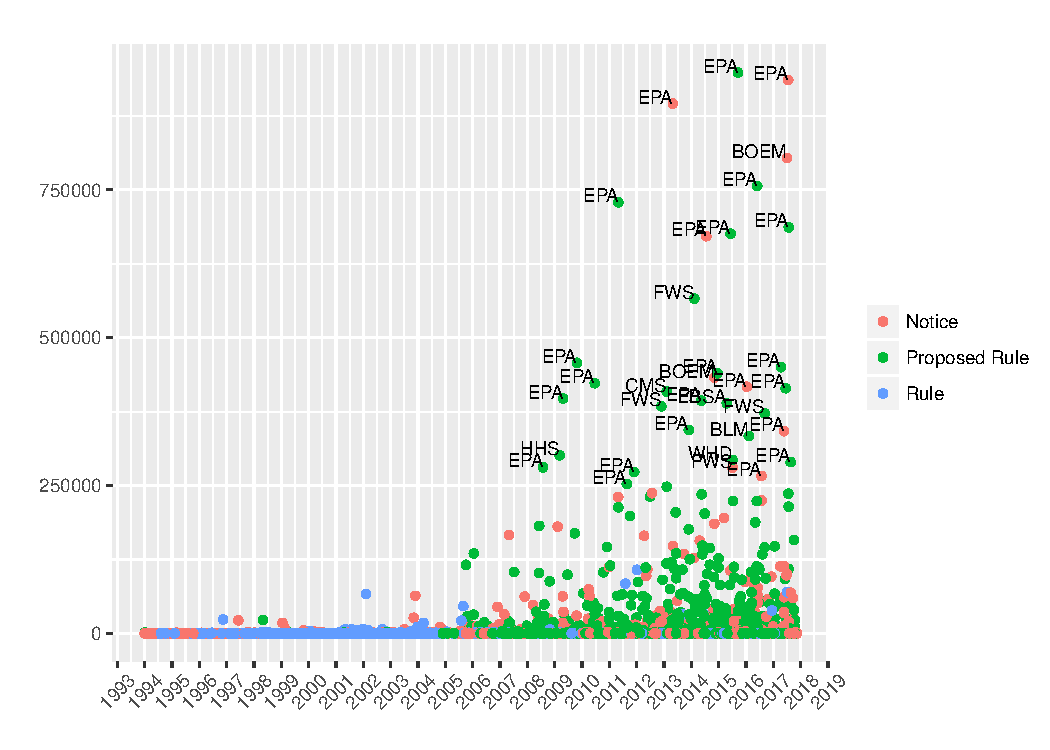
\includegraphics[width = 3.5in]{comments_under_1m.pdf}
\label{fig:comments}
\end{figure}

%It is even less clear whether actions by average citizens make a difference in agency policymaking. Many may believe that they do, but the mechanisms are not obvious. Indeed letter writing and other forms of mass mobilization do not have a clear place in political scientists' theories of bureaucratic politics. This lack of scholarship may be the result of both a general suspicion, rooted in certain theories of strategic behavior, that mass politics affects unelected career officials as well as a normative assumption that policy ``implementation'' is no place for contentious politics. Neither the bureaucrat who asserts that rules are the result of scientific analysis nor the political scientist who asserts that rules are the result of bureaucrats strategically selecting their most preferred policy within institutional constraints offer an explanation for why an agency would receive millions of public comments or why they would matter.











% LEGAL SCHOLARS' DEBATES 
Legal scholars have long debated what to make of mass commenting in rulemaking. Many focus on reforms for agencies to collect more useful information \citep{Farina2011, Farina2014, Rauch2016}. In 2018, ``Public engagement'' was main project of the Administrative Conference of the United States (ACUS) committee on Rulemaking: %\href{https://www.acus.gov/research-projects/public-engagement-rulemaking}
{The project} ''explores agency strategies to enhance public engagement prior to and during informal rulemaking. It seeks to ensure that agencies invest resources in a way that maximizes the probability that rulewriters obtain high quality public information.''  Among other things, this committee is debating how to encourage ``quality public information,'' how ``to get new people/groups into the real or virtual room'' \citep{Farina2018}, and whether broad engagement is even desirable on all rules \citep{White2018}. \citet{Mendelson2011} finds that agencies often discard non-technical comments but argues that they should be given more weight. Others worry that mass commenting distracts agencies from good policy and the broader public interest \citep{Coglianese2006}. \citet[p. 112]{Farina2012} argues that ``[Mass] comments typically are neither factually informative nor reliable indicators of citizens’ informed value preferences.'' \citet{Rossi1997} argues it should be largely eliminated. \citet[p. 208]{Herz2016} concludes ``The goal of e-rulemaking is to more fully capture such credible, specific, and relevant information, not to solicit the views of random, self-nominating members of the public.'' 
Even scholars suggesting reforms aimed at ``regulatory democracy'' aim to increase the ``sophistication'' of ordinary peoples' comments \citep{Cuellar2014}. 

Scholars focusing on deliberation and sophisticated techncial information have overlooked the role importance of political information and representation (but see \citet{Reich1966} and \citet{Seifter2016UCLA} on representation).
Notably, the ACUS draft recommendations on ``Mass and Fake Comments in Agency Rulemaking'' suggests that ``effective comments'' give ``reasons rather than just reactions'' \citep[p. 33]{ACUS2018}. If true, public reactions to proposed rules such as mass comments would have no effect in rulemaking. 

% MAY NOT MATTER 
Like most forms of political participation, 
mass public comments on draft agency rules provide no new technical information. 
They lack the authority of elected officials' opinions. 
And the number on each side has no legal import for an agency's response.
Policymakers may very well pay no attention to them. 

% \subsection{Models of Bureaucratic Politics} 
% MODELS HAVE NO PLACE 
The contentious politics that inspire ordinary people to engage have no place in leading models of bureaucratic policymaking and have largely been ignored by political scientists.
Instead, models focus on how agencies either learn about policy problems, negotiate or avoid accountability to various principals, or balance interest-group demands.\footnote{
On learning, see \citet{Libgober2018} for an information-based model where commenting reveals information to the agency. 

On accountability to elected officials, see  \citet{Furlong1997}, \citet{Nou2016}, \citet{Potter2016}, \citet{Woods2018}, and \citet{Yackee2009RegGov}. For example, \citet{Potter2014dis} presents a signaling model where agencies propose and principals veto rules depending, in part, on their beliefs about interest group preferences. 

On interest group balancing see \citet{Yackee2006JOP},  \citet{Yackee2006JPART}, and \citet{Kerwin2011}.
} 
% SOPHISTICATED LOBBYING
% Influence in rulemaking is sophisticated lobbying efforts of powerful interest groups, whose role in shaping policy has been theoretically developed and empirically tested.

Foundational scholarship on rulemaking by \citet{Furlong2004}, \citet{Furlong1997, Furlong1998}, and \citet{Kerwin2011} focuses on interest group lobbying. Both theory and empirical scholarship suggest skepticism that the input of ordinary people matters. 
% REREAD BERRY
% \citet{Berry1999TheGroups} argues that mass engagement occurs too late in the policy process to be effective compared to insiders who are able to shape agendas and alternatives. 
Empirical scholarship finds that economic elites and business groups dominate American politics in general \citep{Gilens2014} and rulemaking in particular \citep{Crow2015, Wagner2011, West2009, Yackee2006JOP, Yackee2006JPART, Yackee2012, Golden1998, Haeder2015}. Perhaps this is unsurprising. 
From a strategic perspective, agency officials are not directly accountable to voters. And even if organized groups do supplement congressional and judicial checks on executive power, the groups that participate in rulemaking represent only certain (if any) citizens and may not represent them well \citep{Seifter2016UCLA}. Early optimism among legal scholars that the internet would ``change everything'' \citep{Johnson1998} and that ``cyberdemocracy''  would enable more deliberative rulemaking has faded.  Here, the prediction that the internet would merely facilitate engagement among the like-minded \citep{Sunstein2001} has largely been correct. While commenting and encouraging others to comment has become easier, \citet{Coglianese2006} finds that little else has changed. 
From a science-based policy perspective, average citizens signing form letters provide no new information to policymakers. 
Mass comment campaigns are thus often called ``spam'' \citep{Balla2018} and dismissed as epiphenomenal to bargaining with principals or interest groups. 
Yet \citet{Yackee2015JPART} finds that, even though ordinary participants see business influence as more important, they still strongly believe that their comments matter.

% MAIN QUESTION 
% Yet agencies occasionally receive thousands or even millions of comments from ordinary people. %Why? 
\paragraph{Incorperating mass engagement into theories of bureaucratic policymaking.}
How, if at all, should scholars incorporate mass engagement into models of bureaucratic policymaking? 
I argue that mass engagement produces political information about the coalition that mobilized it.
Thus, depending on how agencies process political information, ``going public'' may occasionally be an effective strategy for organizations to influence policy, both directly and indirectly.








%%%%%%%%%%%%%%%%%%%%%%%%%%%%%%%%%%%%%
% % PREVIEW 
% Does mass engagement in bureaucratic policymaking affect policy? This question drives the my project. However, two questions must be answered first: (1) Why does it occur? and (2) How does it affect agencies' political principals? These questions drive two initial empirical chapters. Thus, my analysis has three steps. In step 1, I argue that activists' opportunities and strategies explain variation in engagement. I then ask if this variation in mass engagement explains variation in elected officials' attention (step 2) and on agency responses and policy outcomes (step 3).% But first, I must develop a measure of ``going public.'' % and why it occurs. 

% % PREVIEW EJ AND EXP CHAPTERS 
%The bulk of my project relies on large-n observational data. To explore causal arguments, the last two chapters of the dissertation explore historical and experimental case studies. My historical case is the environmental justice movement, relying on all rules where ``environmental justice'' is raised in the comments and quantitative and qualitative assessment of agency responses. I find that responsiveness varies with with agency missions, but no evidence that the total number of comments affects rules. My experimental cases will be rules selected by organizations that have agreed to randomly assign specific targets of their mass comment campaigns. While these few cases will not provide necessary power for statistical tests, the responses of the public, elected officials may help illuminate causal mechanisms.






% MODEL - regulator is oncertian about backlash 
% org may reveil 
% people react to losses more than gains 
% 262 in 6th eddition - useful thing in identifying diffuse interests - though they may not opposed before - they may mobilize after 



 %While the theory that I assemble attempts to describe the relationship between mass mobilization and agency decisionmaking in general, my empirical focus is on the role of  organized campaigns targeting notice-and-comment rulemaking processes, with special attention to environmental and financial regulation.







